%!TEX TS-program = pdflatex
% prelim.tex -- main prelim file
%
% Wisconsin dissertation template
% Copyright (c) 2008-2009 William C. Benton.  All rights reserved.
%
% This program can redistributed and/or modified under the terms of the LaTeX
% Project Public License Distributed from CTAN archives in directory
% macros/latex/base/lppl.txt; either version 1 of the License, or (at your
% option) any later version.
%
% This program includes other software that is licensed under the terms of the
% LPPL and the Perl Artistic License; see README for details.
%
% You, the user, still hold the copyright to any document you produce with this
% software (like your dissertation).
%

%%% You'll want ``oneside'' for the deposit version, but probably not for any
%%% versions that don't need to meet the UW requirements
\documentclass[12pt,oneside,letterpaper]{memoir}

% preamble.tex -- packages to include
%
% Wisconsin dissertation template
% Copyright (c) 2008 William C. Benton.  All rights reserved.
%
% This program can redistributed and/or modified under the terms
% of the LaTeX Project Public License Distributed from CTAN
% archives in directory macros/latex/base/lppl.txt; either
% version 1 of the License, or (at your option) any later version.
%
% This program includes other software that is licensed under the
% terms of the LPPL and the Perl Artistic License; see README for details.
%
% You, the user, still hold the copyright to any document you produce
% with this software (like your dissertation).

%% Comment out any of these that you don't want
\usepackage{amssymb}
\usepackage{amsmath}
\usepackage{amsthm}
%\usepackage{theorem}
\usepackage{hyperref}

%%%%% LISTINGS package and setup
\IfFileExists{listings.sty}{%
\usepackage{listings}%
}{}

%% Packages added by Matt Gidden
%%
%% Note, order matters!
%%
\usepackage{cite} % right order for multiple entries in cite
\usepackage{moreverb} % for verbatim snippets of code
\usepackage{fancyvrb}
\usepackage{tabularx} % for tables with line breaks
\usepackage{threeparttable} % for tables with notes
\usepackage[capitalize, noabbrev]{cleveref} % for reference multiple figures
\usepackage{calc} % allows for arithmetic on latex variables
\usepackage{float} % allows for figures to be placed explicitly
\usepackage{algorithm2e} % for algorithms
\usepackage{subfig}
\usepackage{multirow} % combining rows in tables
\usepackage{footnote}
\usepackage{titlesec} % for using \titleformat
\usepackage{slashbox} % for tables with a divided cell, see http://tex.stackexchange.com/questions/7262/diagonally-divided-table-cell
\usepackage{bashful}
\usepackage{xspace}
\usepackage{color}
\definecolor{listinggray}{gray}{0.9}
\definecolor{lbcolor}{rgb}{0.9,0.9,0.9}
\lstset{
    %backgroundcolor=\color{lbcolor},
    language={C++},
    tabsize=4,
    rulecolor=\color{black},
    upquote=true,
    aboveskip={1.5\baselineskip},
    belowskip={1.5\baselineskip},
    columns=fixed,
    extendedchars=true,
    breaklines=true,
    prebreak=\raisebox{0ex}[0ex][0ex]{\ensuremath{\hookleftarrow}},
    frame=single,
    showtabs=false,
    showspaces=false,
    showstringspaces=false,
    basicstyle=\scriptsize\ttfamily\color{black},
    keywordstyle=\color[rgb]{0,0,1.0},
    commentstyle=\color[rgb]{0.133,0.545,0.133},
    stringstyle=\color[rgb]{0.627,0.126,0.941},
    numberstyle=\color[rgb]{0,1,0},
    identifierstyle=\color{black},
    captionpos=t,
}
\lstdefinestyle{BashOutputStyle}{
  basicstyle=\small\ttfamily,
  numbers=none,
  frame=tblr,
  columns=fullflexible,
  backgroundcolor=\color{blue!10},
  linewidth=0.9\linewidth,
  xleftmargin=0.1\linewidth
}
%
% Adding for some table features
\usepackage{array}
%
% Adding package for float barriers
\usepackage{placeins}

%% Custom commands added by Matt Gidden
\setcounter{tocdepth}{2}
\setcounter{secnumdepth}{3}
\theoremstyle{plain}
\newcommand{\Cyclopts}{\textsc{Cyclopts} }
\newcommand{\Cycamore}{\textsc{Cycamore} }
\newcommand{\cyclus}{\textsc{Cyclus}\xspace}
\newcommand{\Cyclus}{\textsc{Cyclus} }
\newcommand{\nucl}[2]{
\ensuremath{^{#1}}\mbox{#2}
}
\newcommand{\horizfig}[2][]{%
  \begin{minipage}{3in}\subfloat[#1]{#2}\end{minipage}}
%% \newcommand{\code}[1]{\lstinline[basicstyle=\ttfamily\color{green!40!black}]|#1|}
\newcommand{\code}[1]{\lstinline[basicstyle=\ttfamily\color{black}]|#1|}
\newcommand{\codeb}[1]{\texttt{#1}}
\newcommand{\units}[1] {\:\text{#1}}%
\newcommand{\citeme}{\textcolor{red}{CITE}\xspace}
\newcommand{\TODO}[1] {{\color{red}\textbf{TODO: #1}}}%
\newcommand{\Reactor}[1]{\texttt{Reactor{#1}}}
\newcommand{\UOXSource}{\texttt{UOX\_Source}}
\newcommand{\MOXSource}{\texttt{MOX\_Source}}
\newcommand{\Enrichment}{\texttt{Enrichment}}
\newcommand{\ffc}{$f_{\text{fc}}$\xspace}
\newcommand{\frx}{$f_{\text{rx}}$\xspace}
\newcommand{\floc}{$f_{\text{loc}}$\xspace}
\newcommand{\dloc}{$\delta_{\text{loc}}$\xspace}
\newcommand{\dreg}{$\delta_{\text{reg}}$\xspace}
\newcommand{\cbc}{Cbc\xspace}
\newcommand{\clp}{Clp\xspace}

%% You should use natbib
\IfFileExists{natbib.sty}{%
  \usepackage[numbers]{natbib}% added the numbers option from the original WI
                              % thesis template
}{}

%% You probably need appendix, if you want appendices
\IfFileExists{appendix.sty}{%
\usepackage{appendix}%
}{}

%% the spacing in memoir is weird, you'll need to use this
\DisemulatePackage{setspace}
\usepackage[onehalfspacing]{setspace}

%% List setup; the ``hanglist`` environment will allow you to have
%% nicely-typeset enumerated lists (i.e., with the numbers hanging in
%% the margins).  You need at least version 2.1 of enumitem.sty.  If
%% you don't have enumitem installed at all, hanglist will just be an
%% alias for enumerate.
\IfFileExists{enumitem.sty}{%
\usepackage[loadonly]{enumitem}[2007/06/30]%
\newlist{hanglist}{enumerate}{1}% 
\setlist[hanglist]{label=\arabic*.}%
\setlist[hanglist,1]{leftmargin=0pt}%
}{%
\newenvironment{hanglist}{\begin{enumerate}}{\end{enumerate}}%
}

\IfFileExists{mathpartir.sty}{%
\usepackage{mathpartir}%
}{}

%% \newtheorem{thm}{Theorem}[chapter] % reset theorem numbering for each chapter
%% \theoremstyle{definition}
%% \newtheorem{defn}[thm]{Definition} % definition numbers are dependent on theorem numbers
%% \newtheorem{exmp}[thm]{Example} % same for example numbers


%% Get rid of ugly borders around PDF hyperlinks (e.g., for cross-references, bib entries, or URLs)
\hypersetup{pdfborder = 0 0 0}

%% You want microtype.
\IfFileExists{microtype.sty}{%
\usepackage[protrusion=true,expansion=true]{microtype}%
}{}

%\pagestyle{thesisdraft}

% Surround parts of graphics with box
\usepackage{boxedminipage}

%% booktabs (thx to Nate Rosenblum for bringing this beautiful package
%% to my attention)
\IfFileExists{booktabs.sty}{%
\usepackage{booktabs}%
}{}

% This is now the recommended way for checking for PDFLaTeX:
\usepackage{ifpdf}

%% Avoid ugly "Type 3" fonts
\usepackage{lmodern}
\usepackage[LY1]{fontenc}

%% Substitute your favorite serif and sans fonts here....
\IfFileExists{tgpagella.sty}{%
% TeX Gyre pagella, like Palatino
\usepackage{tgpagella}%
}{}

%% overrides the default Latex math font with AMS Euler
%\usepackage[LY1]{eulervm} 

\ifpdf
\usepackage[pdftex]{graphicx}
\else
\usepackage{graphicx}
\fi

\usepackage{makeidx}
\makeindex

{\theoremstyle{plain}
\newtheorem{thm}{Theorem}[chapter]
\newtheorem{cor}[thm]{Corollary}
\newtheorem{define}[thm]{Definition}
\newtheorem{exmpl}[thm]{Example}
}
{\theoremstyle{remark}
\newtheorem{rmk}[thm]{Remark}
}

\newtheoremstyle{customsty1}
{3pt}%
{3pt}%
{}% --- body font
{}% --- indent amount
{\bfseries}% --- Theorem head font
{:}% --- Punctuation after head
{.5em}% --- space after head
{}% --- theorem head spec (can be left empty, meaning 'normal')

% Define 'newtheorems' that use ``customsty1''
{\theoremstyle{customsty1} 
}


%%% NB: the ``deposit'' chapter- and page- styles should conform to UW
%%% requirements.  If you are producing a pretty version of your
%%% dissertation for web use later, you will certainly want to make
%%% your own chapter and page styles.

\makechapterstyle{deposit}{%
  \renewcommand{\chapterheadstart}{}
  \renewcommand{\printchaptername}{}
  \renewcommand{\chapternamenum}{}
  \renewcommand{\printchapternum}{\parbox{2em}{\MakeLowercase{\Large\scshape\thechapter{}}} }
  \renewcommand{\afterchapternum}{}
  \renewcommand{\printchaptertitle}[1]{%
  \raggedright\Large\scshape\MakeLowercase{##1}}
  \renewcommand{\afterchaptertitle}{%
  \vskip\onelineskip \hrule\vskip\onelineskip}
}

\makepagestyle{deposit}
 
\makeatletter
 
\renewcommand{\chaptermark}[1]{\markboth{#1}{}}
\renewcommand{\sectionmark}[1]{\markboth{#1}{}}
 
\makeevenfoot{deposit}{}{}{}
\makeoddfoot{deposit}{}{}{}
\makeevenhead{deposit}{\thepage}{}{}
\makeoddhead{deposit}{}{}{\thepage}
\makeatother

%%% set up page numbering for chapter pages to satisfy UW requirements
%%% NB: You will want to delete until the ``SNIP'' mark if you are
%%% making a ``nice'' copy
\copypagestyle{chapter}{plain}
\makeoddfoot{chapter}{}{}{}
\makeevenhead{chapter}{\thepage}{}{}
\makeoddhead{chapter}{}{}{\thepage}
%%% SNIP

%%% bib nonsense
\makeatletter
\newenvironment{wb-bib}[1]{%
  \chapter*{references}
\ifnobibintoc\else 
\phantomsection 

\addcontentsline{toc}{chapter}{References } 
\fi 
\prebibhook
  \begin{bibitemlist}{#1}}{\end{bibitemlist}\postbibhook}

\AtBeginDocument{%
  \@ifpackageloaded{natbib}{% natbib is loaded
    \addtodef{\endthebibliography}{}{\vskip-\lastskip\postbibhook}
    \@ifpackagewith{natbib}{sectionbib}{% with sectionbib option
      \renewcommand{\bibsection}{\@memb@bsec}}%
      {\renewcommand{\bibsection}{\@memb@bchap}}}%
  {}
  \@ifpackagewith{chapterbib}{sectionbib}{%
    \renewcommand{\sectionbib}[2]{}
    \renewcommand{\bibsection}{\@memb@bsec}}{}
}
\makeatother

% defs.tex -- wbepi environment for chapter epigraphs and other useful defs.
%
% Wisconsin dissertation template
% Copyright (c) 2008 William C. Benton.  All rights reserved.
%
% This program can redistributed and/or modified under the terms
% of the LaTeX Project Public License Distributed from CTAN
% archives in directory macros/latex/base/lppl.txt; either
% version 1 of the License, or (at your option) any later version.
%
% This program includes other software that is licensed under the
% terms of the LPPL and the Perl Artistic License; see README for details.
%
% You, the user, still hold the copyright to any document you produce
% with this software (like your dissertation).


%% put lstnewenvironment declarations here, if you're using listings

%% end lstnewenvironment declarations

%% I put convenience definitions that will go in several chapters here

%%%%% begin convenience definitions

\makeatletter
\newcommand{\wb@episource}{}
\newenvironment{wbepi}[1]{\begin{quote}\renewcommand{\wb@episource}{#1}\itshape}{\par\upshape \raggedleft --- \textsc{\wb@episource}\\ \end{quote}}
\makeatother

%%%%% SVN
\IfFileExists{svn-multi.sty}{%
\usepackage{svn-multi}%
%%% Uncomment the second one and comment out the first one if you want
%%% to include subversion revision information in each file.
\newcommand{\vcinfo}{}%
%\newcommand{\vcinfo}{\begin{centering}\fbox{\fbox{\parbox{5in}{Author: \svnauthor\\Revision: \svnfilerev\\Last changed on: \svnfiledate\\URL: \svnkw{HeadURL}}}}\\[1em]\end{centering}}%
}{%
\newcommand{\svnidlong}[4]{}%
\newcommand{\svnfilerev}{}%
\newcommand{\svnauthor}{}%
\newcommand{\svnfiledate}{}%
\newcommand{\svnkw}{}%
\newcommand{\vcinfo}{}%
}

%%%%% end convenience definitions

% thesisdefs.tex

% This is mostly adapted from withesis.cls.  The original copyright
% notice for withesis.cls follows, preceded by two percent signs (%%):

%% withesis.cls
%% LaTeX Style file for the University of Wisconsin-Madison Thesis Format
%% Adapted from the Purdue University Thesis Format
%% Originally by Dave Kraynie
%% Edits by Darrell McCauley
%% Adapted to UW-Madison format by Eric Benedict  (Noted with <EB>)
%% Updated to LaTeX2e by Eric Benedict 24 July 00
%% 
%%=============================================================================
%% Licensed under the Perl Artistic License.
%% see: http://www.ctan.org/tex-archive/help/Catalogue/licenses.artistic.html
%% for more info...
%%=============================================================================

% withesis.cls is available from CTAN.  The modifications to this file
% are also licensed under the Perl Artistic License.

% --wb, 2008

\makeatletter

\newcounter {tocpage}
\newcounter {lofpage}
\newcounter {lotpage}
\newcounter {listofheading}

\newcommand\@thesistitlemedskip{0.2in}
\newcommand\@thesistitlebigskip{0.6in}
\newcommand{\degree}[1]{\gdef\@degree{#1}}
\newcommand{\project}{\gdef\@doctype{A masters project report}}
\newcommand{\prelim}{\gdef\@doctype{A preliminary report}}
\newcommand{\thesis}{\gdef\@doctype{A thesis}}
\newcommand{\dissertation}{\gdef\@doctype{A dissertation}}
\newcommand{\department}[1]{\gdef\@department{(#1)}}

\newenvironment{titlepage}
 {\@restonecolfalse\if@twocolumn\@restonecoltrue\onecolumn
  \else \newpage \fi \thispagestyle{empty}
% \c@page\z@ -- deleted: count title page in thesis
}{\if@restonecol\twocolumn \else \newpage \fi}

\gdef\@degree{Doctor of Philosophy}    %Default is PhD
\gdef\@doctype{A dissertation}         %Default is dissertation

\gdef\@department{(Nuclear Engineering and Engineering Physics)}
\gdef\@defensedate{03/26/2015}
\gdef\@committee{
  \hspace*{1cm}Michael L. Corradini, Professor, Nuclear Engineering and Engineering Physics\\
  \hspace*{1cm}James R. Luedtke, Professor, Industrial and Systems Engineering\\
  \hspace*{1cm}Laura A. McLay, Professor, Industrial and Systems Engineering\\
  \hspace*{1cm}Erich A. Schneider, Professor, Nuclear Engineering, University of Texas at Austin\\
  \hspace*{1cm}Paul P.H. Wilson, Professor, Nuclear Engineering and Engineering Physics
  %<+Name+>, <+Title+>, <+Department+>\\
  } 

\renewcommand{\maketitle}{%
  \begin{titlepage}
%-----------------------------------------------------------------------------
% -- The thesis office doesn't like thanks on title page.  Put it in
% -- the acknowledgments.  This is here so you don't have to change
% -- your titlepage when converting from report style. -> from Purdue, but I
%        left it here since it seems compatible with UW-Madison, Eric
%-----------------------------------------------------------------------------
    \def\thanks##1{\typeout{Warning: `thanks' deleted from thesis titlepage.}}
    \let\footnotesize\small \let\footnoterule\relax \setcounter{page}{1}
    \begin{center}
      {\textbf{\expandafter\expandafter{\@title}}} \\[\@thesistitlebigskip]
       by \\[\@thesistitlemedskip]
      \@author \\[\@thesistitlebigskip]
      \@doctype\ submitted in partial fulfillment of \\
      the requirements for the degree of\\[\@thesistitlebigskip]
      \@degree \\[\@thesistitlemedskip]
      \@department \\[\@thesistitlebigskip]
      at the \\[\@thesistitlemedskip]
      UNIVERSITY OF WISCONSIN--MADISON\\[\@thesistitlemedskip]
      \@date
      \\[\@thesistitlemedskip]
    \end{center}
  %% for final thesis
  %% with large margins
  Date of final oral examination: \@defensedate \\[\@thesistitlemedskip]
  The dissertation is approved by the following members of the Final Oral Committee:\\
  %%
  \@committee
  \end{titlepage}
  \setcounter{footnote}{0}
  \setcounter{page}{1} %title page is NOT counted
  \let\thanks\relax
  \let\maketitle\relax \let\degree\relax \let\project\relax \let\dissertation\relax
  \let\department\relax
  \gdef\@thanks{}\gdef\@degree{}\gdef\@doctype{}
  \gdef\@department{}
  %\gdef\@author{}\gdef\@title{}
}


%=============================================================================
% ABSTRACT
%=============================================================================
% The abstract should begin with two single-spaced lines describing
% the author and title in a standard format.  After these lines comes
% the standard abstract.
%=============================================================================
\def\abstract{
  \chapter*{Abstract}
  \addcontentsline{toc}{chapter}{Abstract}
  \relax\markboth{Abstract}{Abstract}}
\def\endabstract{\par\newpage}


%=============================================================================
% UMI ABSTRACT
%=============================================================================
% The UMI abstract should begin with the author and title in a standard format.
% After the author comes the advisor and university. After these lines comes
% a bunch of double spaced text to make up the standard abstract.
% After the abstract, the advisor's approval signature follows.
% This page is not numbered and is delivered seperately to the thesis office.
%=============================================================================

\def\advisortitle#1{\gdef\@advisortitle{#1}}
\def\advisorname#1{\gdef\@advisorname{#1}}
\gdef\@advisortitle{Professor}
\gdef\@advisorname{Cheer E.\ Place}

\def\umiabstract{
             \thispagestyle{empty}
                  \addtocounter{page}{-1}
                \begin{center}
                  {\textbf{\expandafter\uppercase\expandafter{\@title}}}\\
                  \vspace{12pt}
                  \@author \\
                  \vspace{12pt}
                  Under the supervision of \@advisortitle\ \@advisorname\\
                  At the University of Wisconsin-Madison
                \end{center}
}

\def\endumiabstract{\vfill \hfill\@advisorname\par\newpage}


%============================================================================
% VERBATIMFILE
%============================================================================
% \verbatimfile{<filename>}    for verbatim inclusion of a file
% - Note that the precise layout of line breaks in this file is important!
% - added the \singlespace - EB
%============================================================================
\def\verbatimfile#1{\begingroup \singlespace
                    \@verbatim \frenchspacing \@vobeyspaces
                    \input#1 \endgroup
}


%=============================================================================
% SEPARATOR Pages
%   Creates a blank page with a text centered horizontally and vertically.
%   The page is neither counted nor numbered.
%   These pages are required in the thesis format before sections such
%   as appendices, vita, bibliography, etc.
%=============================================================================
\def\separatorpage#1{
  \newpage
  \thispagestyle{empty}
  \addtocounter{page}{-1}
  \null
  \vfil\vfil
  \begin{center}
    {\textbf{#1}}
  \end{center}
  \vfil\vfil
  \newpage}


%=============================================================================
% COPYRIGHTPAGE
%=============================================================================
% The copyright must do the following:
% - start a new page with no number
% - place the copyright text centered at the bottom.
%=============================================================================
\def\copyrightpage{
  \newpage
  \thispagestyle{empty}    % No page number
  \addtocounter{page}{-1}
  \chapter*{}            % Required for \vfill to work
  \begin{center}
   \vfill
   \copyright\ Copyright by \@author\ \@date\\
   All Rights Reserved
  \end{center}}


%=============================================================================
% GLOSSARY
%=============================================================================
% The glossary environment must do the following:
% - produce the table of contents entry for the glossary
% - start a new page with GLOSSARY centered two inches from the top
%=============================================================================
\def\glossary{
  \chapter*{GLOSSARY}
  \addcontentsline{toc}{chapter}{Glossary}}
\def\endglossary{\par\newpage}

%=============================================================================
% NOMENCLATURE
%=============================================================================
% The nomenclature environment must do the following:
% - produce the table of contents entry for the nomenclature section
% - start a new page with NOMENCLATURE centered two inches from the top
%=============================================================================
\def\nomenclature{\separatorpage{DISCARD THIS PAGE}
  \chapter*{Nomenclature}
  \addcontentsline{toc}{chapter}{NOMENCLATURE}}
\def\endnomenclature{\par\newpage}

%=============================================================================
% CONVENTIONS
%=============================================================================
% The conventions environment must do the following:
% - produce the table of contents entry for the nomenclature section
% - start a new page with CONVENTIONS centered two inches from the top
%=============================================================================
\def\conventions{\separatorpage{DISCARD THIS PAGE}
  \chapter*{Conventions}
  \addcontentsline{toc}{chapter}{CONVENTIONS}}
\def\endconventions{\par\newpage}


%=============================================================================
% COLOPHON
%=============================================================================
% The colophon environment must do the following:
% - produce the table of contents entry for the nomenclature section
% - start a new page with COLOPHON centered two inches from the top
%=============================================================================
\def\colophon{\separatorpage{DISCARD THIS PAGE}
  \chapter*{Colophon}
  \addcontentsline{toc}{chapter}{Colophon}}
\def\endcolophon{\par\newpage}

%=============================================================================
% LIST OF SYMBOLS
%=============================================================================
% The list of symbols environment must do the following:
% - produce the table of contents entry for the list of symbols section
% - start a new page with LIST OF SYMBOLS centered two inches from the top
%=============================================================================
\def\listofsymbols{\separatorpage{DISCARD THIS PAGE}
  \eject
  \chapter*{LIST OF SYMBOLS}
  \addcontentsline{toc}{chapter}{LIST OF SYMBOLS}}
\def\endlistofsymbols{\par\newpage}

%=============================================================================
% VITA
%=============================================================================
% The vita environment must do the following:
% - produce a separator page with the word vita centered
% - produce the table of contents entry for the vita
% - start a new page with VITA centered two inches from the top
%=============================================================================
\def\vita{
%  \separatorpage{VITA}         % UW doesn't require this EB
  \chapter*{VITA}
  \addcontentsline{toc}{chapter}{VITA}}
\def\endvita{\par\newpage}

%=============================================================================
% ACKNOWLEDGMENTS
%=============================================================================
% The acknowledgments environment must do the following:
% - start a new page with ACKNOWLEDGMENTS centered two inches from the top
%=============================================================================
\def\acks{
  \chapter*{Acknowledgments}
}
\def\endacks{\par\newpage}

%=============================================================================
% DEDICATION
%=============================================================================
% The dedication environment must do the following:
% - start a new page
% - center the text vertically
% - include the text in a center environment
%=============================================================================
\def\dedication{
  \newpage
  \null\vfil
  \begin{center}}
\def\enddedication{\end{center}\par\vfil\newpage}

%=============================================================================
% DATE
%=============================================================================
%\def\today{\ifcase\month\or
  %January\or February\or March\or April\or May\or June\or
  %July\or August\or September\or October\or November\or December\fi
  %\space\number\day, \number\year}
\newcount\@testday
\def\today{\@testday=\day
  \ifnum\@testday>30 \advance\@testday by -30
  \else\ifnum\@testday>20 \advance\@testday by -20
  \fi\fi
  \number\day\ \
  \ifcase\month\or
    January \or February \or March \or April \or May \or June \or
    July \or August \or September \or October \or November \or December
    \fi\ \number\year
}


%  Single counter for theorems and theorem-like environments:
\newtheorem{theorem}{Theorem}[chapter]
\newtheorem{assertion}[theorem]{Assertion}
\newtheorem{claim}[theorem]{Claim}
\newtheorem{conjecture}[theorem]{Conjecture}
\newtheorem{corollary}[theorem]{Corollary}
\newtheorem{definition}[theorem]{Definition}
\newtheorem{example}[theorem]{Example}
\newtheorem{figger}[theorem]{Figure}
\newtheorem{lemma}[theorem]{Lemma}
\newtheorem{prop}[theorem]{Proposition}
\newtheorem{remark}[theorem]{Remark}

%=============================================================================
% TABLE OF CONTENTS; LIST OF FIGURES; LIST OF TABLES
%=============================================================================
% In report style, \tableofcontents, \listoffigures, etc. are always
% set in single-column style.  @restonecol is used to keep track of
% whether we need to switch back to double column style after the toc.
%
% The only known problem now is that the first page with the new
% layout is too long.  The problem seems to be that the change to
% textheight doesn't take place on the first page.  Even if it's the
% first line in the table of contents macro.  Presumably the same
% problem also occurs in the lof and lot.
%
% I'm taking a shot at fixing the problem by dropping in a throw-away
% page between the change to the height parameters and the start of
% the chapter.  Isn't elegance wonderful?
%
%=============================================================================

% \def\@tableof#1#2#3#4#5{
% { % limit scope of following declarations!!
%   \@restonecolfalse\if@twocolumn\@restonecoltrue\onecolumn\fi
%   \addtolength{\textheight}{-40pt}       % -24-16
%   \addtolength{\majorheadskip}{-40pt}    % -24-16
%   \addtolength{\headheight}{52pt}        %  36+16
%   \addtolength{\headsep}{-12pt}          % -12
%   \separatorpage{DISCARD THIS PAGE}
%   \chapter*{#1}
%   #5
%   \relax\markboth{#1}{#1}
%   \hbox to \hsize{#2 \hfil Page}
%   \singlespace
%   \setcounter{#3}{0}
%   \setcounter{listofheading}{1}  % change from 0 to 1 by mccauley, 14may93
%   \def\@oddhead{\vbox to \headheight{\vspace{4pt}
%     \hbox to \hsize{\hfil\textrm{\thepage}} \vfil
%     \ifnum\value{#3}=1
%       \ifnum\value{listofheading}=2
%         \hbox to \hsize{Appendix\hfil} \vspace{4pt} \fi
%       \ifnum\value{listofheading}=1
%         \stepcounter{listofheading} \fi
%       \hbox to \hsize{#2 \hfil Page}
%     \else
%       \setcounter{#3}{1}
%     \fi}}
%   \def\@evenhead{\vbox to \headheight{\vspace{4pt}
%     \hbox to \hsize{\textrm{\thepage}\hfil} \vfil
%     \ifnum\value{#3}=1
%       \ifnum\value{listofheading}=2
%         \hbox to \hsize{Appendix\hfil} \vspace{4pt} \fi
%       \ifnum\value{listofheading}=1
%         \stepcounter{listofheading} \fi
%       \hbox to \hsize{#2 \hfil Page}
%     \else
%       \setcounter{#3}{1}
%     \fi}}
%   \@starttoc{#4}  \if@restonecol\twocolumn\fi
%   \newpage
% }}
% 
% \def\tableofcontents{\@tableof{TABLE OF CONTENTS}{}{tocpage}{toc}{}}
% 
% \def\listoffigures{
%   \@tableof{LIST OF FIGURES}{Figure}{lofpage}{lof}
%   {\protect\addcontentsline{toc}{chapter}{LIST OF FIGURES}}}
% 
% \def\listoftables{
%   \@tableof{LIST OF TABLES}{Table}{lotpage}{lot}
%   {\protect\addcontentsline{toc}{chapter}{LIST OF TABLES}}}

%=============================================================================
% BIBLIOGRAPHY
%=============================================================================
% The thebibliography environment executes the following commands:
%
%  o start a new 'chapter' with BIBLIOGRAPHY as the heading
%  o produce a separator page for the bibliography
%
%  \def\newblock{\hskip .11em plus .33em minus -.07em} --
%      Defines the `closed' format, where the blocks (major units of
%      information) of an entry run together.
%
%  \sloppy  -- Used because it's rather hard to do line breaks in
%      bibliographies,
%
%  \sfcode`\.=1000\relax --
%      Causes a `.' (period) not to produce an end-of-sentence space.
%=============================================================================
% \altbibtitle
%   The default title for the References chapter is ``LIST OF REFERENCES''
%   Since some people prefer ``BIBLIOGRAPHY'', the command
%   \altbibtitle has been added to change the chapter title.
%   This command does nothing more than change REFERENCES to BIBLIOGRAPHY
%============================================================================
\def\@bibchaptitle{Bibliography}
\def\altbibtitle{\def\@bibchaptitle{Bibliography}}
\def\thebibliography#1{
  %\separatorpage{\@bibchaptitle}
  \global\@bibpresenttrue
  \chapter*{\@bibchaptitle\markboth{\@bibchaptitle}{\@bibchaptitle}}
  \addcontentsline{toc}{chapter}{\@bibchaptitle}
  \vspace{0.375in}    % added to match 4 line requirement
  \interlinepenalty=10000 % added to prevent breaking of bib entries
  \singlespace\list
  {[\arabic{enumi}]}{\settowidth\labelwidth{[#1]}\leftmargin\labelwidth
    \advance\leftmargin\labelsep \usecounter{enumi}}
  \def\newblock{\hskip .11em plus .33em minus -.07em}
  \sloppy
  \sfcode`\.=1000\relax}
\let\endthebibliography=\endlist



\makeatother

\svnidlong{$LastChangedBy$}{$LastChangedRevision$}{$LastChangedDate$}{$HeadURL: http://freevariable.com/dissertation/branches/diss-template/dissertation.tex $} 

\clearpage\pagenumbering{roman}  % This makes the page numbers Roman (i, ii, etc)

\title{An Agent-Based Modeling Framework and Application for the Generic Nuclear
  Fuel Cycle}
\author{Matthew J.~Gidden}
\department{Nuclear Engineering \& Engineering Physics}
\prelim

\date{2013}

\begin{document}

%%% Uncomment the following if your .bib contains references that you will not 
%%% explicitly cite, but that should be in the final bibliography:
% \nocite{*}

\ifpdf
\DeclareGraphicsExtensions{.pdf, .jpg, .tif}
\else
\DeclareGraphicsExtensions{.eps, .jpg}
\fi

\maketitle

%% Add \part declarations if you want, but it's not necessary
%\part{Preliminaries}

%% frontmatter includes dedication, acknowledgements, TOC, List of Tables, List
%% of Figures, umiabstract, abstract
%\svnidlong{$LastChangedBy$}{$LastChangedRevision$}{$LastChangedDate$}{$HeadURL: http://freevariable.com/dissertation/branches/diss-template/frontmatter/frontmatter.tex $}
%\vcinfo{}

%%% SOME OF THIS CODE IS ADAPTED FROM THE VENERABLE withesis.cls

% COPYRIGHT PAGE
%  - To include a copyright page use \copyrightpage
\copyrightpage

% DEDICATION
\begin{dedication}
  \emph{This work is dedicated to my parents, Howard and Melanie, who always
believed that I could do anything I set my mind to, and to Ms. Margaret Maes,
who has been my solid foundation through the highs and lows of the past few
years.}
\end{dedication}

%% BEGIN PAGESTYLE

%%% You can pick a pagestyle if you want; see the memoir class
%%% documentation for more info.  The default ``deposit'' option meets
%%% the UW thesis typesetting requirements but is probably
%%% unsatisfactory for making a version of your dissertation that
%%% won't be deposited to the graduate school (e.g., for web or a nice
%%% printed copy)

\chapterstyle{deposit}
\pagestyle{deposit}


% ACKNOWLEDGMENTS
\begin{acks}
% \begin{wbepi}{David C.~Makinson (1965)}
%   It is customary for authors of academic books to include in their prefaces
%   statements such as this: ``I am indebted to ... for their invaluable help;
%   however, any errors which remain are my sole responsibility.'' Occasionally
%   an author will go further. Rather than say that if there are any mistakes
%   then he is responsible for them, he will say that there will inevitably be
%   some mistakes and he is responsible for them....

%   Although the shouldering of all responsibility is usually a social ritual,
%   the admission that errors exist is not --- it is often a sincere avowal of
%   belief. But this appears to present a living and everyday example of a
%   situation which philosophers have commonly dismissed as absurd; that it is
%   sometimes rational to hold logically incompatible beliefs.
% \end{wbepi}

Ceci n'est pas un Acknowledgement.

\end{acks}

% CONTENTS, TABLES, FIGURES
\renewcommand{\printtoctitle}[1]{\chapter*{#1}}
\renewcommand{\printloftitle}[1]{\chapter*{#1}}
\renewcommand{\printlottitle}[1]{\chapter*{#1}}

\renewcommand{\tocmark}{}
\renewcommand{\lofmark}{}
\renewcommand{\lotmark}{}

\renewcommand{\tocheadstart}{}
\renewcommand{\lofheadstart}{}
\renewcommand{\lotheadstart}{}

\renewcommand{\aftertoctitle}{}
\renewcommand{\afterloftitle}{}
\renewcommand{\afterlottitle}{}

\renewcommand{\cftchapterfont}{\normalfont} 
\renewcommand{\cftsectionfont}{\itshape} 
\renewcommand{\cftchapterpagefont}{\normalfont} 
\renewcommand{\cftchapterpresnum}{\bfseries} 
\renewcommand{\cftchapterleader}{} 
\renewcommand{\cftsectionleader}{} 
\renewcommand{\cftchapterafterpnum}{\cftparfillskip} 
\renewcommand{\cftsectionafterpnum}{\cftparfillskip} 

% \captionnamefont{\small\sffamily} 
% \captiontitlefont{\small\sffamily} 

% \renewcommand{\contentsname}{contents}
% \renewcommand{\listfigurename}{list of figures}
% \renewcommand{\listtablename}{list of tables}

\tableofcontents

\clearpage
\listoftables

\clearpage
\listoffigures

\clearpage
% NOMENCLATURE
% \begin{conventions}
% % \begin{description}
% % \item{\makebox[0.75in][l]{term}
% %        \parbox[t]{5in}{definition\\}}
% % \end{description}
% \input{conventions}
% \end{conventions}

\advisorname{Paul P.~H.~Wilson}
\advisortitle{Professor}

% ABSTRACT
%% \begin{umiabstract}
%%   Ceci n'est pas un Abstract. \cite{guerin_benchmark_2009}

%% \end{umiabstract}
\begin{abstract}
  Ceci n'est pas un Abstract. \cite{guerin_benchmark_2009}

\end{abstract}

\clearpage\pagenumbering{arabic}

%%% END STUFF TAKEN FROM WITHESIS EXAMPLE FILE


%% Now include the tex files for each chapter, like so (I put these in separate
%% dirs):
This chapter seeks to lay out a plan by which a fully agent-based simulation can
be implemented for a generic nuclear fuel cycle with a more realistic chemical
separations and fuel-matching model than currently exists in the field. The term
generic implies that the facilities involved are not known \textit{a priori}
and, accordingly, facilities can be coupled together automatically, separating
the concern of fuel facility modeling and connection from the simulation
solution engine. For example, a modeler has the choice to model a separations
facility and advanced fuel fabrication facility as separate entities whose
connected supply and demand are met by a generic engine, or to model the two
facilities as a single combined and coupled entity. Additionally, the solution
framework for this matching engine must be agnostic as to the classes of
commodities and materials involved. Rather than hard-coding in constraints and
capacities for different material classes, they are added dynamically based on
the entities involved in the simulation-based solution.

As fuel cycle simulators have progressed from simple spreadsheet applications,
work advancing the field has focused on including in-simulation dynamic
calculations of important metrics and parameters in order to provide feedback to
the simulation rather than solely post-processing simulation output. A number of
examples exist. COSI uses the CESAR depletion code \cite{vidal_cesar:_2006} to
automate output fuel characteristics in order to reduce voluminous user input
for simulated materials. Scopatz introduced the notion of essential physics
modeling with his Bright simulation engine \cite{scopatz_essential_2011}. Most
recently, Huff has added to this area of work by developing a repository
facility for the \Cyclus simulator that analyzes repository effects due to
different combinations of materials in different repository
geologies~\cite{huff_integrated_2013}.

This work proposes additional advancement of the dynamic simulation of nuclear
fuel cycles using the \Cyclus simulator. First, a simulation framework for
simulation entity interaction is introduced, the primary goal of which is to
encapsulate simulation-level design decisions. The framework allows for market
interactions to be defined, providing a formalism by which information related
to supply and demand of commodities and materials can be represented in a
general sense. Commodities are not treated simply as quantities, instead the
quantity and \textit{quality} of commodities is treated.  Next, a mathematical
programming formulation based on the multi-commodity transport problem is
proposed to solve the generic supply-demand matching problem. A linear program
formulation and mixed integer-linear program formulation is proposed, the latter
of which addresses the trade-off between computation speed and realism. Finally,
the issue of matching separated elemental streams with requested recycled fuel
is addressed via an approximation linear program.

% 
\begin{frame}[ctb!]
  \frametitle{FCS History}

  \begin{columns}[t]

    \column{.33\textwidth}
    \begin{block}{Spreadsheets}
      \begin{itemize}
        \item very inextensible
        \item basic output
        \item little to no decision making
      \end{itemize}
    \end{block}

    \pause

    \column{.33\textwidth}
    \begin{block}{Simulation Dynamics}
      \begin{itemize}
        \item limited extensibility
        \item aggregate mass flows
        \item limited \textit{in situ} decision making
        \item fleet based
      \end{itemize}
    \end{block}

    \pause

    \column{.33\textwidth}
    \begin{block}{Next Generation FCS}
      \begin{itemize}
        \item extensible
        \item \textit{in situ} decision making
        \item isotopic-based dynamics
        \item facility-level effects
        \item region-level effects
      \end{itemize}
    \end{block}

  \end{columns}
  
\end{frame}

\begin{frame}[ctb!]
  \frametitle{Issues with Current SD Implementations}
  
  \begin{itemize}
    \item fleet-based models lack facility-level detail (e.g., facility
      disruptions, facility location, transportation, etc.)
    \item aggregate mass flows lack isotopic-level detail
    \item static facility (fleet) connections
    \item equation-based model limits simulation extensibility
    \item little-to-no recycled fuel matching fidelity
  \end{itemize}

\end{frame}

\begin{frame}[ctb!]
  \frametitle{Basic \Cyclus Approach}

  \begin{itemize}
    \item treat facilities individually
    \item facilities discretely transact materials
    \item materials are defined by both an isotopic \textit{quality} and
      quantity
    \item designed with extensibility in mind
  \end{itemize}

\end{frame}

\begin{frame}[ctb!]
  \frametitle{Making \Cyclus Extensible}
  
  Facilities, materials (i.e., commodities) are treated generally in \Cyclus.

  \begin{figure}
    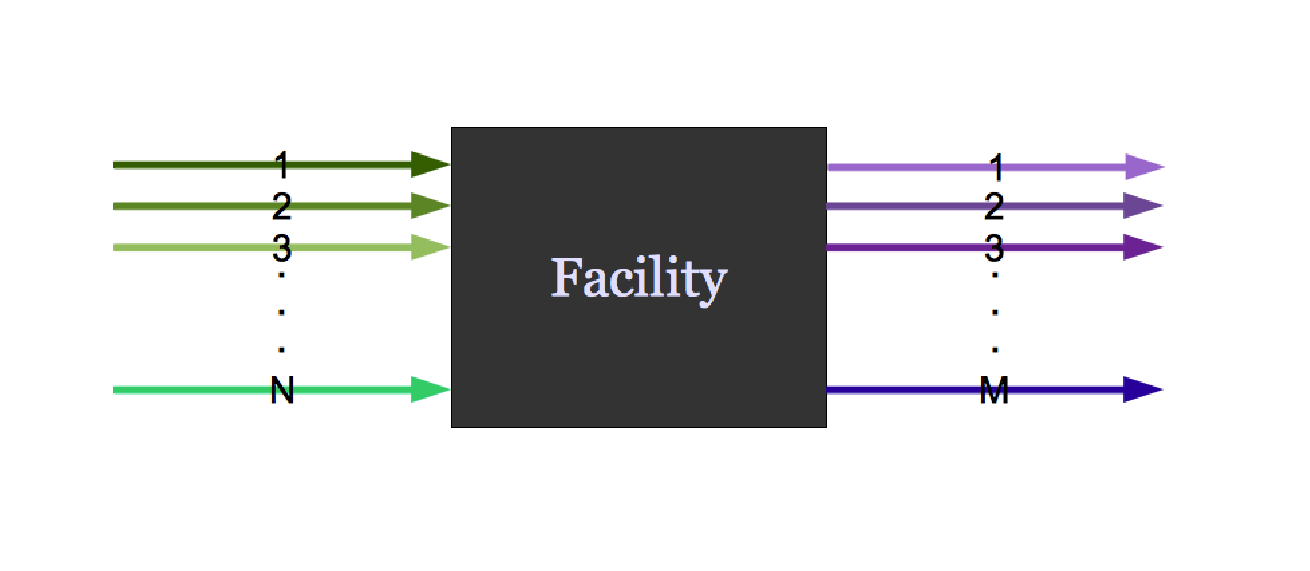
\includegraphics[height=4cm]{./images/facs.eps}
    \caption{Facilities as black boxes. \cite{cyclus2012}.}
    \label{fig:facs}  
  \end{figure}

\end{frame}

\begin{frame}[ctb!]
  \frametitle{Issues with Current Recycled Fuel Matching}
  
  Current implementations of the modeling of recycled fuel fabrication
  \begin{itemize}
    \item lack rigor
    \item don't account for element-isotope issues present at this interface
  \end{itemize}
  
  \vspace{0.2cm}

  VISION models the process by:
  \begin{itemize}
    \item placing separated isotopes in ``bins''
    \item declaring ``control isotopes''
    \item removing the correct control isotopes fraction from the bin
  \end{itemize}
  
\end{frame}

\begin{frame}[ctb!]
  \frametitle{Issues with Current Recycled Fuel Matching}

  COSI's uses the ``Equivalence Model'', adapted from a method introduced in
  1963 by Baker and Ross\cite{baker_comparison_1963}.
  
  \vspace{0.2cm}

  Method and implementation outline:
  \begin{itemize}
    \item used for recycled fuel recipes
    \item assumes ``ideal'' recipe of $^{239}$Pu and $^{238}$U
    \item determines a recipe given ``bins'' of fissile and fertile material
  \end{itemize}
\end{frame}

\begin{frame}[ctb!]
  \frametitle{Issues with Current Recycled Fuel Matching}

  In such a model, the following are defined:
  \begin{itemize}
    \item a quantity of fuel
    \item a target Pu-239 enrichment, $E_0$
    \item a ``bin'' of fertile isotopes
    \item a ``bin'' of fissile isotopes
  \end{itemize}

  And its output is:
  \begin{itemize}
    \item a weight fraction, $E$, to extract from the fissile isotopes
    \item a weight fraction, $1-E$, to extract from the fertile isotopes
  \end{itemize}
\end{frame}

\begin{frame}[ctb!]
  \frametitle{Issues with Current Recycled Fuel Matching}
  
  An isotopic ``worth'' is defined for each isotope, $i$, as:
  \begin{equation}
    w_i = \frac{x_i - x_{^{238}U}}
    {x_{^{239}Pu} - x_{^{238}U}}.
  \end{equation}

  with $x_i$ defined as:
  
  \begin{equation}
    x_i = \nu_{i} \sigma_{f,i} - \sigma_{a,i}
  \end{equation}

  with physical parameters:
  \begin{itemize}
    \item $\nu_{i}$ - average number of neutrons resulting from fission
    \item $\sigma_{f,i}$ - microscopic fission cross section
    \item $\sigma_{a,i}$ - microscopic absorption cross section
  \end{itemize}
\end{frame}

\begin{frame}[ctb!]
  \frametitle{Issues with Current Recycled Fuel Matching} 
  
  With isotopic weight fractions, $\xi_i$, the fissile fraction, $E$, is given
  by:
  \begin{equation}
    E = \frac{E_0 - \sum_{i \in I_{Fe}} \xi_i w_i}
    {\sum_{i \in I_{Fi}} \xi_i w_i - \sum_{i \in I_{Fe}} \xi_i w_i}.
  \end{equation}

  \begin{figure}
    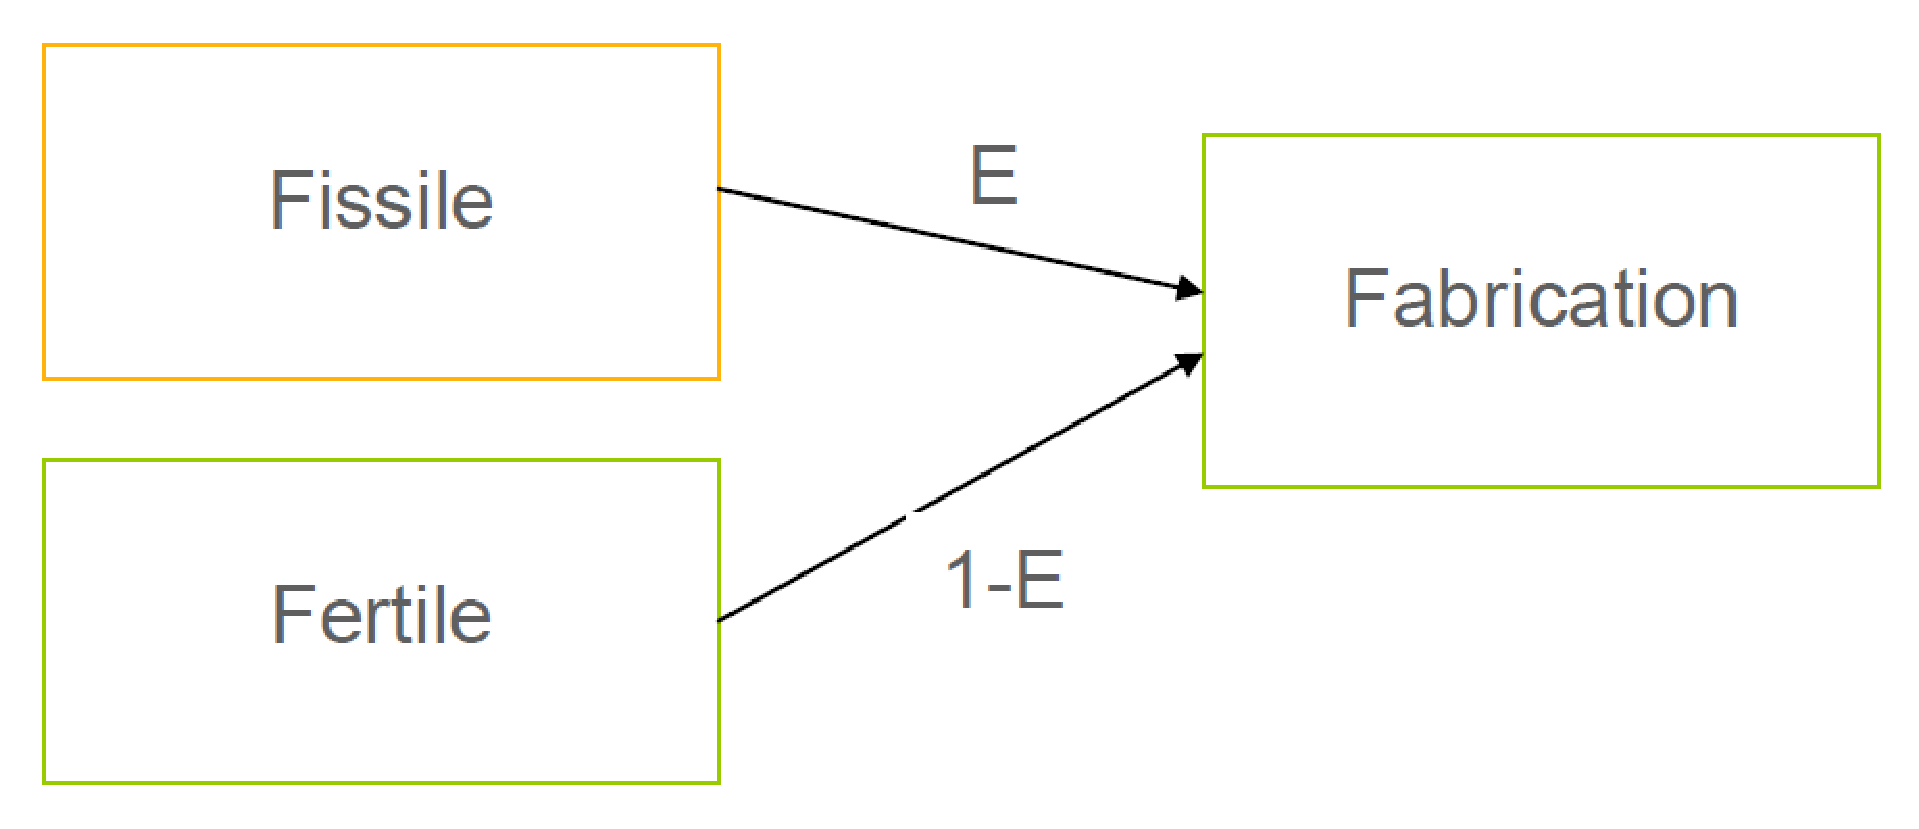
\includegraphics[height=3cm]{./images/equiv.eps}
    \caption{Result of COSI's Equivalence Method. \cite{meyer_new_2009}.}
  \end{figure}
\end{frame}
  
\begin{frame}[ctb!]
  \frametitle{Two Motivating Questions}

  \begin{block}{Dynamic Resource Exchange}
    If facilities are treated as individual black boxes and connections between
    facilities are determined dynamically, how does one match suppliers with
    demanders considering supply constraints and, supply response to
    quality-based demands, and issues of fungibility?
  \end{block}

  \pause

  \begin{block}{Fuel Order Approximation}
    Can one model the interface between separations and recycled fuel
    fabrication more realistically?
  \end{block}

\end{frame}

% \include{related/related}

%% etc, etc.

%% Do you have appendices?  If so, add them here, just like chapters.
% \begin{appendices}
% \chapter{\Cyclus To Date}\label{sec:cyclus}

Significant, strategic improvements have been added to the \Cyclus code base.
Interactions with dynamically-loadable libraries and reading XML-input files
have been encapsulated in classes and enhanced. 

\section{Dynamic Loading}\label{sec:prev-dynamic}

Software libraries can be accessed in a static manner, i.e., they are connected
to an application during the linking phase of building a program, or can be
accessed in a dynamic manner, i.e., they are connected at run time. Dynamic
linkage, or dynamic loading, is a well-known technique for to support
connectable, modular components, or plug-ins. \Cyclus utilizes a plug-in
approach for its facility, institution, and region agent libraries. This design
decision furthers the \Cyclus development goal of providing an agnostic
framework into which sophisticated users can develop different models of agents
to investigate specific simulation-modeling change.

Work was performed in order to use class-based representation of dynamic
libraries, allowing for easy opening, closing, and access thereof. Each dynamic
library represents an agent type in \Cyclus, providing a constructor and
destructor. The DynamicModule class then provides the \Cyclus core access to
these constructors and destructors to perform the appropriate operations at run
time. Because dynamic loading is treated differently on POSIX-based systems than
it is on Windows-based systems, specialty functions for library access were
provided for each system. The correct header file (UnixHelperFunctions.h or
WindowsHelperFunctions.h) is chosen during compilation. 

These changes simplified the client code that utilizes library access. The
\Cyclus core application can now call appropriate library-related functions in
an agnostic manner. Specific, well-defined time points of module loading
(dynamic library opening) and unloading (dynamic library closing) were defined
in the \Cyclus application. These operations, called by the application,
currently reside in the Model class and could likely be refactored into a
specific handler class designed for this purpose.

\section{Input Reading}

A large overhaul to the input-reading code base was performed. \Cyclus currently
only supports XML input files that adhere to the RNG schema defined in the
\Cyclus RNG file. However, it is a well-known best practice to provide an
agnostic application programming interface (API) that can be configured with
specific class instances given some user-defined input. Accordingly, such an API
was constructed which currently supports XML input but can also support future
input types that are tree-based (e.g., JSON, CSV, etc.).

The top-level abstraction is encased in a QueryEngine class. Basic operations
are provided assuming a tree-based input formation, including querying the
number of child elements at the current reading level, the name of each element,
and access to each element. The application code is responsible for configuring
the appropriate input parser and populating an instance of a QueryEngine at its
root. The client code then populates input parameters through the QueryEngine
interface rather than an input-format specific interface.

Support for XML-file reading has been enhanced by separating various concerns
into appropriate classes. Four classes have been constructed with specific
purposes regarding input file reading: file loading (XMLFileLoader), file
validation (RelaxNGValidator), file parsing (XMLParser), and querying
(XMLQueryEngine). The application interfaces with the file loader, initializing
it with a given input file path and then invoking the loading of various
\Cyclus-specific parameters (e.g., simulation control parameters, material
recipes, agent modules, etc.). The loader is responsible for managing its parser
and providing client code with correctly-configured instances of
XMLQueryEngines. The parser is responsible for providing an interface to the
underlying C++ XML parsing library (i.e., libxml++) and invoking the appropriate
validation routines on the parsed file. The validator is responsible for
providing access to the RNG-validation operations through libxml and
libxml++. Finally, the XML-specific derived QueryEngine class is responsible for
implementing XML querying using the generic QueryEngine interface.

Other input file formats can be supported by providing the appropriate
format-specific derived QueryEngine class and adjusting the application code as
necessary. A developer could then choose how to implement the loading and
validation, if any, of the input file. The structure described above is just one
of many ways to achieve such a goal.

% \end{appendices}

%% Are you a big nerd with a colophon?  Add it here.
% \begin{colophon}
% %\svnidlong{$LastChangedBy$}{$LastChangedRevision$}{$LastChangedDate$}{$HeadURL: http://freevariable.com/dissertation/trunk/frontmatter.tex $}
%\vcinfo{}

This template uses Gyre Pagella by default.  (I used Arno Pro in my dissertation.)

Feel free to give me a shout-out in your colophon or acks if this template is useful for you.  Good luck!

% \end{colophon}

%% McBride is a very nice style (some version is included in this distribution)
\bibliographystyle{mcbride}
\bibliography{refs}

%% Want an index?  Neither did I.
%\printindex

\end{document}
